%
% supersonic.tex -- the equation for a supersonic flow
%
% (c) 2008 Prof Dr Andreas Mueller
%
\rhead{Supersonic flow}
\section{Supersonic flow}
In the year 1928, Jakob Ackeret habilitated at ETH Zürich with a 
\index{Ackeret, Jakob}
\index{supersonic flow}
paper with the title
``Über Luft-Kräfte bei sehr grossen
Geschwindigkeiten insbesondere bei ebenen Strömungen''.
He showed how to compute the aerodynamic forces on an object
in a supersonic flow using a linear approximation.
The velocity field of the gas that enters the region of interest with
velocity $v_1$ in $x$-direction turns out to be the gradient of
a function $\varphi(x,y,z)$ that satisfies the equation
\[
(1-\textit{Ma}_1)\frac{\partial^2\varphi}{\partial x^2}
+
\frac{\partial^2\varphi}{\partial y^2}
+
\frac{\partial^2\varphi}{\partial z^2}=0.
\]
The expression
$\textit{Ma}_1=\frac{v_1}{c_1}$ is called the Mach number of the flow,
$c_1$ is the speed of sound.
The Mach number expresses the flow velocity in units of the speed of sound.

For small velocities, we have $(1-\textit{Ma}_1)>0$, and the equation
becomes similar to the Poisson problem.
This is called potential flow.

\begin{figure}
\begin{center}
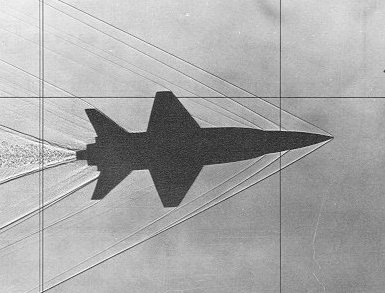
\includegraphics[width=0.8\hsize]{../common/graphics/i-5-1}
\end{center}
\caption{Flow around a supersonic plane\label{examples:ueberschall2d}}
\end{figure}

For supersonic flow, however, the first term
$(1-\textit{Ma}_1) < 0$
changes sign, and the equation behaves like a wave equation.
In fact, the flow shows shock waves propagating away from the object
and thus carrying away its energy
(figure~\ref{examples:ueberschall2d}).
By carefully analyzing this solution, Ackeret was able to compute
aerodynamic drag due to these shock waves.
\index{aerodynamic drag}
\index{shock waves}

